\section{Symulacyjne wyznaczenie odpowiedzi skokowej procesu}
Wyznaczyc symulacyjnie odpowiedzi skokowe procesu dla kilku zmian sygnału sterujacego,
przy uwzglednieniu ograniczen wartosci tego sygnału, jego wartosc na poczatku
eksperymentu wynosi Upp. Narysowac te odpowiedzi na jednym rysunku. Narysowac
charakterystyke statyczna procesu y(u). Czy własciwosci statyczne i dynamiczne procesu
sa (w przyblizeniu) liniowe? Jezeli tak, okreslic wzmocnienie statyczne procesu.

\begin{figure}[H]
    \centering
    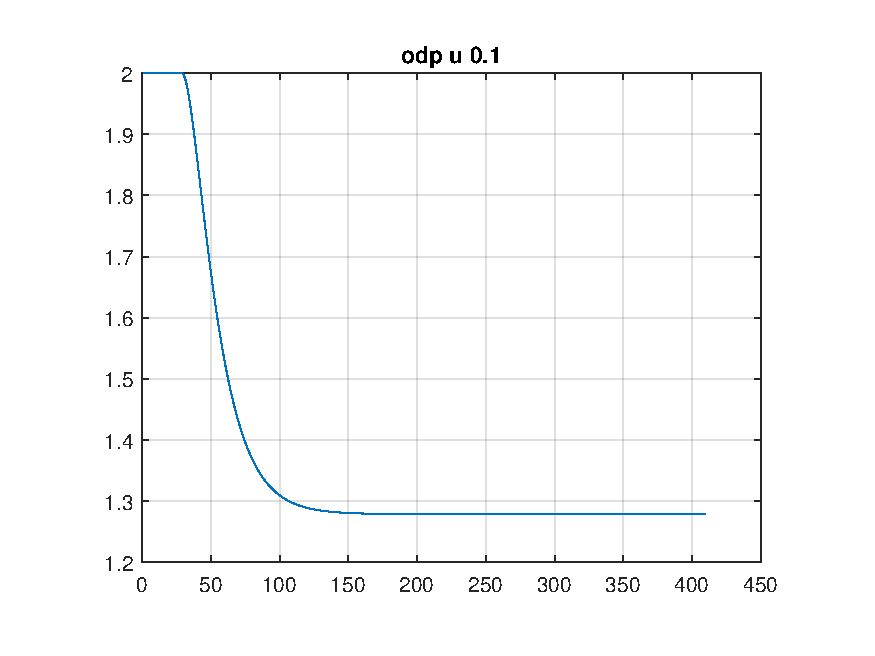
\includegraphics[scale=0.8]{../zad2/img/odp_u_0_1.pdf}
    \caption{rysuneczek 1}
\end{figure}
\begin{figure}[H]
    \centering
    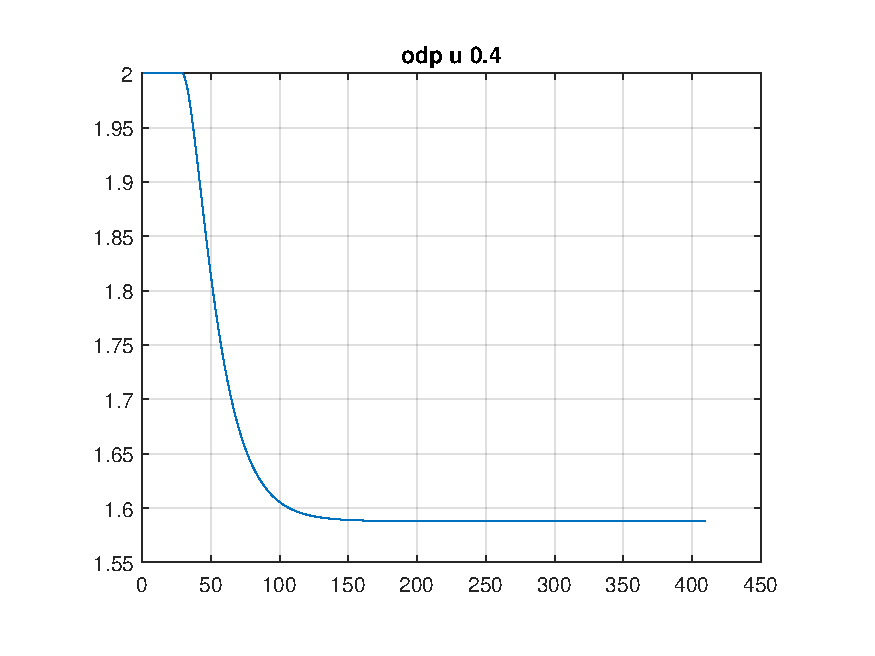
\includegraphics[scale=0.8]{../zad2/img/odp_u_0_4.pdf}
    \caption{rysuneczek 2}
\end{figure}
\begin{figure}[H]
    \centering
    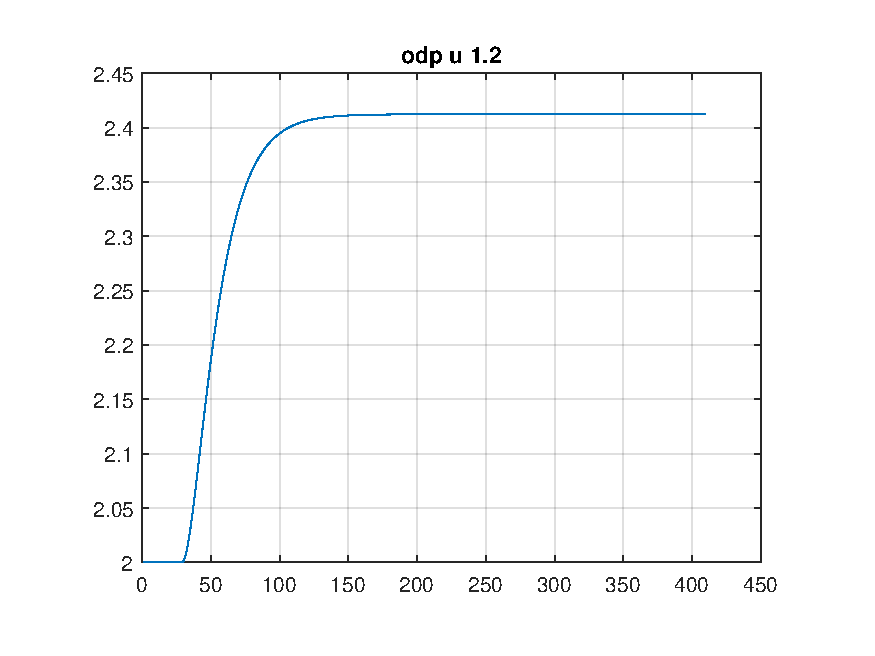
\includegraphics[scale=0.8]{../zad2/img/odp_u_1_2.pdf}
    \caption{rysuneczek 3}
\end{figure}
\begin{figure}[H]
    \centering
    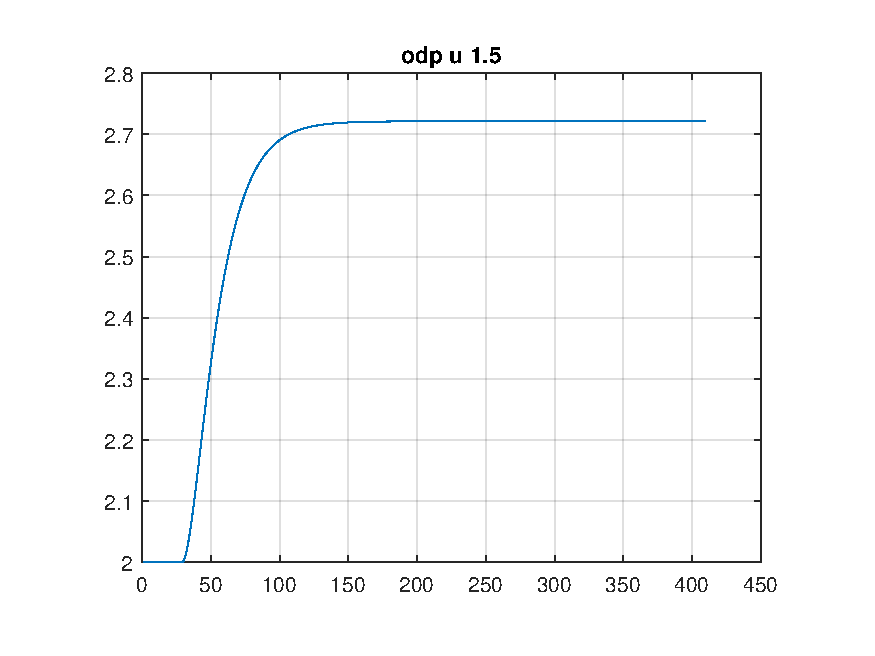
\includegraphics[scale=0.8]{../zad2/img/odp_u_1_5.pdf}
    \caption{rysuneczek 4}
\end{figure}
